% Analisi Matematica II -- Lezione 5
% Teorema di Abel, serie derivata e serie integrale, serie di Taylor, funzioni analitiche.
% Frammento da includere con \input: niente preambolo.
% La numerazione delle figure di questa lezione parte da 14.
\setcounter{figure}{13}

% [0:01:03]
\section{Richiami sulle serie di potenze}

Delle serie di potenze $\sum_{n=0}^{\infty} a_n x^n$ abbiamo scoperto che convergono sempre almeno in un
punto (il punto iniziale): l'insieme di convergenza puntuale, che indichiamo con $\overline{\underline{X}}$, non è mai vuoto.
Anzi, se non si riduce al solo punto iniziale, $\overline{\underline{X}}$ è addirittura un \emph{intervallo}, limitato o illimitato, e
in entrambi i casi è sempre \emph{simmetrico rispetto al punto iniziale}; la sua semiampiezza $\rho$ è il
\emph{raggio di convergenza}. Si hanno tre casi:
\begin{itemize}
  \item $\rho = 0 \ \Rightarrow\ \overline{\underline{X}} = \{0\}$;
  \item $\rho = +\infty \ \Rightarrow\ \overline{\underline{X}} = \mathbb{R}$;
  \item $\rho \in \,]0,+\infty[ \ \Rightarrow\ \overline{\underline{X}} \supseteq \,]{-\rho},\rho[$, e gli estremi $x=\pm\rho$ vanno
        studiati a parte.
\end{itemize}

La domanda rimasta in sospeso era: \emph{come si determina $\rho$?}
% [0:02:28]
Se per trovarlo dovessimo studiare la serie di funzioni non guadagneremmo nulla. Invece $\rho$ si calcola con il
criterio della radice o con quello del rapporto, che nel caso delle serie di potenze si chiamano
\emph{criterio di Cauchy--Hadamard} e \emph{criterio di d'Alembert}:
\[
  \frac{1}{\rho} = \lim_{n\to\infty} \sqrt[n]{|a_n|}
  \qquad\text{oppure}\qquad
  \frac{1}{\rho} = \lim_{n\to\infty} \frac{|a_{n+1}|}{|a_n|} .
\]
A seconda del numero che si ottiene si cade in uno dei tre casi precedenti.

% [0:03:49]
Non solo sappiamo chi è l'insieme di convergenza, ma sappiamo anche caratterizzare il \emph{tipo} di
convergenza: se $0<\rho<+\infty$ la convergenza è assoluta in $]{-\rho},\rho[$ e totale in ogni compatto
$[-r,r]$ con $0<r<\rho$ (Teorema~1). Nessuno di questi teoremi, però, dice nulla negli estremi: che l'intervallo
si chiuda o meno dipende dall'esercizio che si ha davanti, e non si può fare una teoria generale. Quello che si
può dire in generale è che cosa si \emph{guadagna} come tipo di convergenza se l'intervallo si chiude in un
estremo: è il contenuto del teorema di Abel.

% [0:05:15]
\subsection{Teorema di Abel}

\paragraph{Teorema (di Abel, senza dimostrazione).}
Sia $\sum_{n=0}^{\infty} a_n x^n$ una serie di potenze e sia $\rho$, con $0<\rho<+\infty$, il suo raggio di
convergenza. Se la serie converge in $x=\rho$ (oppure in $x=-\rho$), cioè se converge la serie numerica
$\sum a_n \rho^n$ (oppure $\sum a_n (-\rho)^n$), allora la serie converge uniformemente in ogni intervallo del
tipo $[s,\rho]$ (oppure $[-\rho,s]$), con $-\rho<s<\rho$. Se converge sia in $x=\rho$ sia in $x=-\rho$, allora
converge uniformemente in tutto il compatto $[-\rho,\rho]$.

% [0:05:15]
Si considera direttamente il caso di raggio finito e non nullo perché negli altri due casi ($\rho=0$,
$\rho=+\infty$) non c'è niente da dire sugli estremi. Esistono molti altri risultati legati alla convergenza
negli estremi, ma il corso si limita a questo.

\paragraph{Osservazione.}
Abel permette di studiare la convergenza uniforme senza passare necessariamente per la convergenza totale.

\paragraph{Esempio.}
Studiamo la serie
\[
  \sum_{n=1}^{\infty} \frac{(-1)^n}{n}\, x^n , \qquad a_n = \frac{(-1)^n}{n} .
\]
% [0:09:15]
Per trattarla come serie di potenze bisogna prima individuare $a_n$ e $x^n$; la serie è già centrata nel punto
giusto ($x_0=0$), quindi si passa subito al raggio di convergenza. Con Cauchy--Hadamard:
\[
  \frac{1}{\rho} = \lim_{n\to\infty} \sqrt[n]{\left|\frac{(-1)^n}{n}\right|}
  = \lim_{n\to\infty} \frac{1}{\sqrt[n]{n}} = 1
  \quad\Longrightarrow\quad \rho = 1 .
\]
Dunque la serie converge puntualmente (e assolutamente) in $]{-1},1[$ e totalmente in ogni $[-r,r]$ con
$0<r<1$. Che cosa si può dire della convergenza uniforme?

% [0:10:49]
Se la consegna chiede di studiare la convergenza \emph{uniforme}, l'esercizio non è finito: dal Teorema~1 e dal
criterio di Weierstrass (la totale implica l'uniforme) si ottiene l'uniforme solo nei compatti simmetrici
$[-r,r]$; se invece l'intervallo si chiude da qualche parte, bisogna vedere se si può applicare altro, cioè Abel.
In pratica si devono studiare due serie numeriche, ottenute sostituendo $x=-1$ e $x=1$:
\begin{itemize}
  \item per $x=-1$:
        $\displaystyle \sum_{n=1}^{\infty} \frac{(-1)^n}{n}(-1)^n = \sum_{n=1}^{\infty} \frac{1}{n}$,
        la serie armonica, divergente: da questo lato l'intervallo \emph{non si chiude};
  \item per $x=1$: $\displaystyle \sum_{n=1}^{\infty} \frac{(-1)^n}{n}$, la serie armonica a segni alterni,
        che converge per il criterio di Leibniz.
\end{itemize}
% [0:14:34]
Qui le due serie numeriche sono note, ma in generale può servire un criterio di Analisi~I (il termine generale
che non tende a zero, il criterio della radice, \dots): chi pensava di essersi lasciato le serie numeriche alle
spalle se le ritrova.

% [0:15:38]
Riassumendo, grazie ad Abel si può rispondere completamente:
\begin{center}
\begin{tabular}{ll}
  \hline
  tipo di convergenza & insieme \\
  \hline
  puntuale   & $]{-1},1]$ \\
  assoluta   & $]{-1},1[$ \quad (in $x=1$ la serie dei moduli è l'armonica) \\
  totale     & $[-r,r]$, con $0<r<1$ \quad (Teorema~1) \\
  uniforme   & $[s,1]$, con $-1<s<1$ \quad (Abel) \\
  \hline
\end{tabular}
\end{center}

% [0:16:58]
\subsection{Serie di potenze non centrate nell'origine}

Un suggerimento per gli esercizi: una serie di potenze non centrata nell'origine si tratta con un
\emph{cambio di variabile}, che la riconduce alla forma canonica centrata in $0$.

\paragraph{Esempio.}
Consideriamo
\[
  \sum_{n=1}^{\infty} \frac{(x-1)^n}{n^2} ,
\]
una serie di potenze centrata in $x_0=1$. Con la sostituzione $y = x-1$ si ottiene $\sum_{n=1}^{\infty}
\frac{y^n}{n^2}$. Calcoliamo il raggio con il criterio del rapporto (o della radice) sui coefficienti
$a_n = 1/n^2$:
\[
  \lim_{n\to\infty} \frac{|a_{n+1}|}{|a_n|} = \lim_{n\to\infty} \frac{n^2}{(n+1)^2} = 1
  \quad\Longrightarrow\quad \rho = 1 .
\]
% [0:16:58]
Con la radice si trova lo stesso risultato, perché $\sqrt[n]{n^2} = \bigl(\sqrt[n]{n}\bigr)^2 \to 1$: serie di
questo tipo hanno quasi tutte raggio~$1$.

La serie converge internamente per $y\in\,]{-1},1[$. Controlliamo gli estremi:
\begin{itemize}
  \item per $y=1$ ($x=2$): $\displaystyle\sum_{n=1}^{\infty} \frac{1}{n^2}$, armonica generalizzata con
        esponente $2>1$: converge (assolutamente);
  \item per $y=-1$ ($x=0$): $\displaystyle\sum_{n=1}^{\infty} \frac{(-1)^n}{n^2}$: converge assolutamente.
\end{itemize}

% [0:18:24]
\paragraph{Osservazione.}
È un consiglio, non una regola: se $a_n>0$ conviene controllare prima l'estremo positivo $y=\rho$. Se lì la serie
converge, poiché i termini sono positivi la convergenza è assoluta, e allora la serie converge anche in
$y=-\rho$, dove la serie dei moduli è la stessa. Qui, ad esempio, $\sum 1/n^2$ è proprio la serie dei moduli di
$\sum (-1)^n/n^2$: non serve nemmeno Leibniz. Con $(-1)^n$ Leibniz è immediato, ma in casi più complicati sfruttare
l'assoluta convergenza evita lavoro.

L'intervallo si chiude in entrambi gli estremi. Poiché $|y^n/n^2| \le 1/n^2$ per $|y|\le 1$ e
$\sum 1/n^2$ converge, in $y$ la convergenza è puntuale, uniforme e totale in $[-1,1]$.
% [0:19:37]
L'esercizio però non è finito: bisogna tornare alla variabile $x$ risolvendo la disequazione
\[
  -1 \le y \le 1 \iff -1 \le x-1 \le 1 \iff 0 \le x \le 2 .
\]
Per $x$ l'intervallo di convergenza puntuale, uniforme e totale è quindi $[0,2]$, centrato in $1$.

% [0:22:02]
\section{Continuità, derivazione e integrazione della somma}

% [0:22:02]
I termini $a_n x^n$ di una serie di potenze sono potenze: si possono derivare quante volte si vuole, e $a_n$ non
dipende da $x$. È questo il motivo per cui interessa il passaggio al limite sotto il segno di serie: se si può
applicare il teorema di derivazione per serie, lo si può riapplicare alla derivata prima, poi alla seconda, e
così via, e si scopre che la somma è di classe $C^\infty$.

% [0:22:56]
\subsection{Continuità della somma}

Supponiamo che una serie di potenze abbia raggio di convergenza $\rho>0$ e sia
\[
  \sum_{n=0}^{\infty} a_n x^n = S(x) \qquad \text{in } ]{-\rho},\rho[ .
\]
Possiamo dire qualcosa sulla continuità della somma? Dov'è continua $S$?

$S$ è continua in tutto $]{-\rho},\rho[$. Infatti, per il Teorema~1, ogni volta che ci si mette in un compatto
$[-r,r]\subset\,]{-\rho},\rho[$ la convergenza è totale, quindi uniforme; poiché i termini $a_n x^n$ sono continui,
$S$ è continua in ogni compatto.
% [0:22:56]
Gli estremi $\pm\rho$ non si prendono mai, ma i compatti si possono allargare quanto si vuole, avvicinandosi agli
estremi: il fatto che l'intervallo sia aperto permette ogni volta di prendere la convergenza totale in un compatto
sempre più grande, e ogni punto di $]{-\rho},\rho[$ sta in uno di questi compatti (figura~\ref{fig:14}).

\begin{figure}[htbp]\centering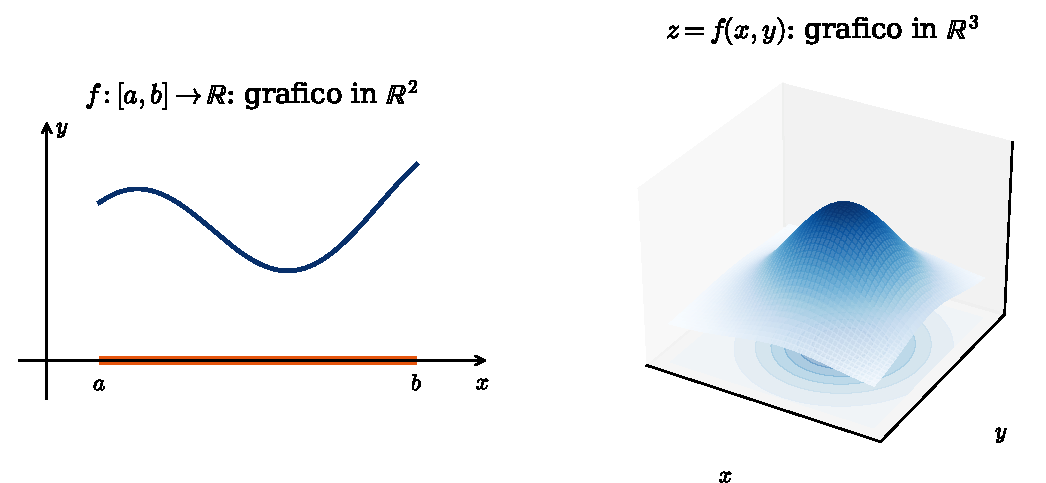
\includegraphics[width=0.6\linewidth]{figure/fig_14}\caption{Compatti $[-r,r]$
sempre più grandi contenuti nell'intervallo aperto $]{-\rho},\rho[$: in ciascuno la convergenza è totale e la
somma $S$ è continua (ricostruzione dello schema degli appunti, p.~3).}\label{fig:14}\end{figure}

Per Abel, se ci sono le condizioni, la serie converge anche negli estremi.
% [0:24:11]
In quel caso la convergenza uniforme arriva fino all'estremo, e con essa la continuità: la somma eredita il
dominio di continuità esattamente dal dominio di convergenza. Ci possiamo chiedere ora che cosa accade alla
derivabilità, che è più delicata, perché il teorema di derivazione per serie ha ipotesi più complesse di quello
di continuità. Per prima cosa bisogna capire chi è la \emph{serie derivata}; poi si considererà anche la
\emph{serie integrale}.

% [0:25:22]
\subsection{Serie derivata}

Consideriamo
\[
  \sum_{n=0}^{\infty} a_n x^n = a_0 + a_1 x + a_2 x^2 + \dots + a_n x^n + \dots
\]
e deriviamola termine a termine.
% [0:25:22]
Il termine noto $a_0$ è costante e sparisce, quindi la serie derivata perde un indice e parte da $n=1$; $a_n$
resta costante e la derivata di $x^n$ è $n x^{n-1}$ (l'esponente scende davanti). La \emph{serie derivata} è
\[
  \sum_{n=1}^{\infty} n\, a_n x^{n-1} .
\]
Posto $b_n = n a_n$,
\[
  \sum_{n=1}^{\infty} b_n x^{n-1} = \sum_{n=0}^{\infty} b_{n+1} x^n ,
\]
cioè abbiamo ottenuto di nuovo una serie di potenze.
% [0:26:29]
Che il coefficiente sia $b_{n+1}$ invece di $b_n$ non ha importanza: chiamandolo $c_n = b_{n+1}$ si vede che è
sempre una successione, e la serie derivata è della stessa natura di quella di partenza.

Per usare il teorema di derivazione per serie bisogna capire dove la serie derivata converge uniformemente, e
quindi trovarne il raggio di convergenza.
% [0:27:37]
Ha senso chiedersi se si può passare al limite sotto il segno di derivata per le serie di potenze prendendo
l'intersezione tra l'intervallo di convergenza della serie madre e quello della serie derivata; la prima cosa da
vedere è quindi che cosa succede al raggio.

\paragraph{Proposizione.}
Sia $\sum a_n x^n$ una serie di potenze e sia $\sum n a_n x^{n-1}$ la sua serie derivata. Allora le due serie
hanno lo stesso raggio di convergenza.

% [0:28:59]
Dimenticando la sua provenienza, la serie derivata è una serie di potenze nuova: a sua volta ha una serie
derivata, $\sum n(n-1) a_n x^{n-2}$, la serie delle derivate seconde, e così via. Dimostrato il risultato per la
derivata prima, vale per tutte le derivate: è il punto di partenza per capire che chiedersi il passaggio al
limite è ragionevole, perché l'insieme in cui convergono è lo stesso.

\paragraph{Dimostrazione.}
Siano $\rho$ il raggio della serie madre e $\tilde\rho$ quello della serie derivata. Per Cauchy--Hadamard
\[
  \frac{1}{\rho} = \lim_{n\to\infty} \sqrt[n]{|a_n|} ,
  \qquad
  \frac{1}{\tilde\rho} = \lim_{n\to\infty} \sqrt[n]{|n a_n|}
  = \lim_{n\to\infty} \sqrt[n]{n}\cdot\sqrt[n]{|a_n|} = 1\cdot\frac{1}{\rho} ,
\]
perché $\sqrt[n]{n}\to 1$. Quindi $\tilde\rho = \rho$.
% [0:32:10]
(C'è un piccolo abuso di notazione: la serie derivata ha la potenza $x^{n-1}$, quindi a rigore l'indice
andrebbe spostato di uno, ma il limite non cambia.)

Il raggio, e quindi l'intervallo aperto di convergenza, della serie derivata non cambia: nell'intervallo di
convergenza della serie ha sempre senso chiedersi se vale il passaggio sotto il segno di derivata. Il discorso
è diverso per la serie integrale.

% [0:32:10]
\subsection{Serie degli integrali}

Nel teorema di integrazione per serie integravamo in un intervallo $[a,b]$: così però si ottiene una serie di
numeri, che non è più una serie di potenze.
% [0:33:36]
Per avere che anche la serie degli integrali sia una serie di potenze non si integra tra $a$ e $b$, ma si usa la
\emph{funzione integrale}: si prende $x$ nell'insieme di convergenza (sempre con $\rho>0$) e si integra su
$[0,x]$, che è un particolare intervallo $[a,b]$.

Data $\sum_{n=0}^{\infty} a_n x^n$, integriamo in $[0,x]$ con $|x|<\rho$; per non confondere la variabile di
integrazione con l'estremo $x$, la chiamiamo $t$. La \emph{serie delle funzioni integrali} è
\[
  \sum_{n=0}^{\infty} a_n \int_0^x t^n\,dt ,
\]
dove $a_n$, costante, è stato portato fuori dall'integrale. Poiché
$\int_0^x t^n\,dt = \bigl[\tfrac{t^{n+1}}{n+1}\bigr]_0^x = \tfrac{x^{n+1}}{n+1}$, si ottiene
\[
  \sum_{n=0}^{\infty} a_n \frac{x^{n+1}}{n+1} = \sum_{n=1}^{\infty} a_{n-1} \frac{x^n}{n} ,
\]
cioè abbiamo ottenuto di nuovo una serie di potenze.

La serie di partenza è la serie derivata di questa nuova serie: derivando $a_n \frac{x^{n+1}}{n+1}$ si ritrova
$a_n x^n$.
% [0:37:35]
Non serve quindi un altro teorema: per la proposizione precedente le due serie hanno lo stesso raggio. Serie
madre, serie derivata e serie integrale hanno tutte lo stesso raggio di convergenza.

% [0:37:35]
\subsection{Teoremi di derivazione e integrazione per serie di potenze}

% [0:37:35]
Per le serie di potenze i teoremi di derivazione e di integrazione per serie si scrivono esattamente come per le
serie di funzioni, ma senza richiedere ipotesi aggiuntive: si applicano all'interno di $]{-\rho},\rho[$, dove la
convergenza è uniforme in tutti i compatti, e allargando i compatti si arriva a tutto l'intervallo aperto, come
per la continuità di $S$.

\paragraph{Teorema (derivazione per serie di potenze).}
Sia $\sum_{n=0}^{\infty} a_n x^n$ una serie di potenze e sia $S(x)$ la sua somma in $]{-\rho},\rho[$, con
$\rho>0$. Allora $S$ è derivabile in $]{-\rho},\rho[$ e risulta
\[
  S'(x) = \sum_{n=1}^{\infty} n\, a_n x^{n-1} \qquad \text{in } ]{-\rho},\rho[ .
\]
% [0:38:44]
L'ipotesi $\rho>0$ è necessaria: se $\rho=0$ la somma è definita in un solo punto e non ha senso derivarla.
% [0:40:13]
Il teorema dice solo che $S$ è derivabile, ma $S'$ è anche continua, cioè $S\in C^1$, perché $S'$ è a sua volta
la somma di una serie di potenze. Le ipotesi del teorema generale sono tutte automatiche: le $f_n$ sono
polinomi, quindi di classe $C^1$, e si sa già che la serie derivata converge ``bene'' nello stesso intervallo.

\paragraph{Teorema (integrazione per serie di potenze).}
Sia $\sum_{n=0}^{\infty} a_n x^n$ una serie di potenze con $\rho>0$ e sia $S(x)$ la sua somma. Allora, per ogni
$x\in\,]{-\rho},\rho[$,
\[
  \sum_{n=0}^{\infty} a_n \frac{x^{n+1}}{n+1} = \int_0^x S(t)\,dt .
\]

% [0:44:17]
\paragraph{Osservazione (calcolo di somme).}
Conseguenza immediata di questi due teoremi, usatissima negli esercizi: tutti i ``parenti'' della serie
geometrica $\sum_{n=0}^{\infty} x^n = \frac{1}{1-x}$ ($|x|<1$), cioè tutte le serie ottenute da essa con
derivate o integrali, diventano serie di cui si sa calcolare la somma. Quando l'esercizio chiede di
\emph{calcolare la somma}, la serie va vista come parente di una geometrica: se $n$ sta a numeratore si tratta di
derivate (per esempio $n^2$ fa pensare alla derivata seconda della geometrica), se sta a denominatore si tratta
di integrali.

% [0:43:00]
\subsection{Esercizio svolto}

Determinare l'insieme di convergenza e calcolare la somma della serie
\[
  \sum_{n=1}^{\infty} n\, x^n .
\]
La serie è parente della serie geometrica, quindi la somma è calcolabile: la vediamo come derivata della serie
geometrica (è ciò che si fa ogni volta che viene chiesto di calcolare la somma).

% [0:45:21]
\emph{Insieme di convergenza.} È la parte più semplice: $\sqrt[n]{n}\to 1$, quindi $\rho=1$; negli estremi
$x=\pm1$ il termine generale $n(\pm1)^n$ non tende a zero, quindi non si chiude nulla. L'insieme di convergenza
è $]{-1},1[$, come per la geometrica.

\emph{Regolarità.} La somma è derivabile in $]{-1},1[$.
% [0:45:21]
Iterando il teorema di derivazione, ``come un programma'', si ottiene di più: riapplicandolo alla serie derivata
si scopre che anche $S'$ è derivabile, e così via, quindi la somma è di classe $C^\infty(]{-1},1[)$.

\emph{Somma.}
% [0:46:37]
Si porta fuori una $x$, in modo che resti esattamente la serie derivata della geometrica (con esponente $n-1$);
il termine $n=0$ si può aggiungere perché la derivata della costante $x^0=1$ è nulla:
\begin{align*}
  \sum_{n=1}^{\infty} n\, x^n
  &= x \sum_{n=1}^{\infty} n\, x^{n-1}
  = x \sum_{n=0}^{\infty} \frac{d}{dx}\bigl(x^n\bigr)
  = x\, \frac{d}{dx} \Bigl( \sum_{n=0}^{\infty} x^n \Bigr) \\
  &= x\, \frac{d}{dx} \Bigl( \frac{1}{1-x} \Bigr)
  = \frac{x}{(1-x)^2} ,
  \qquad x\in\,]{-1},1[ .
\end{align*}
% [0:49:46]
Se si preferisce lasciare la somma da $n=1$, bisogna ricordare che $\sum_{n=1}^{\infty} x^n = \frac{1}{1-x}-1$:
il termine tolto si sottrae, e comunque la derivata non lo vede. In alternativa si poteva integrare subito per
eliminare la $n$ (serie integrale) e poi derivare di nuovo: è una scelta.

% [0:51:03]
Il docente accenna anche a una serie [?] il cui coefficiente va scomposto in fratti semplici, come somma di due
frazioni con $n-1$ e $n+1$: ciascun pezzo diventa una serie integrale, e nell'insieme di convergenza si ottengono
due somme finite.

% [0:55:58]
\paragraph{Attenzione all'indice iniziale.}
È l'unico punto in cui è facile sbagliare: una serie parte da $1$, un'altra da $0$, e se i conti non tornano
bisogna togliere (o aggiungere) pezzi alla somma.
% [0:57:13]
Per sapere se una serie numerica converge non importa perdere qualche termine, ma per calcolarne la somma serve
tutta l'espressione: un termine dimenticato va rimesso.

% [0:51:03]
\subsection{Serie riconducibili a serie di potenze}

Prendiamo la serie
\[
  \sum_{n=1}^{\infty} \frac{(-1)^n (\log x)^n}{n^3+1} , \qquad x\in[1,+\infty[ .
\]
Possiamo studiarla come una serie di potenze?
% [0:52:18]
Come per $(x-1)^n$ si fa la sostituzione $y=x-1$, che è una traslazione, così si può sostituire anche una
funzione di $x$: basta dimenticarsi chi è quel ``signore'' e chiamarlo $y$.
Poniamo $y=-\log x$: poiché $(-1)^n(\log x)^n = (-\log x)^n = y^n$, la serie si riscrive come serie di potenze
\[
  \sum_{n=1}^{\infty} \frac{y^n}{n^3+1} .
\]
Questa serie va studiata in tutti i suoi aspetti:
\begin{itemize}
  \item convergenza puntuale;
  \item convergenza uniforme (all'interno, e con Abel fino agli estremi se l'intervallo si chiude);
\end{itemize}
si ottengono così gli intervalli in $y$, e da lì partono le disequazioni per passare poi in $x$.
% [0:54:58]
La parte di Analisi~II dell'esercizio finisce con il calcolo di $\rho$ (che è un limite) e lo studio degli
estremi; da lì comincia un esercizio di Analisi~I sulle disequazioni. Se è possibile determinare la somma della
serie in $y$, si trova anche la somma della serie di partenza sostituendo.

% [0:53:40]
\paragraph{Attenzione.}
La sostituzione funziona perché la dipendenza da $x$ non si mescola con $n$.
% [0:57:13]
Se nella sostituzione $y=\dots$ si mette dentro una $n$, è un errore gravissimo: $y$ può dipendere solo da $x$.
% [0:58:39]
Per esempio
\[
  \sum_{n=1}^{\infty} \frac{\bigl(\log(x+n)\bigr)^n}{n^3+n}
\]
non si può ricondurre a una serie di potenze, perché dentro il logaritmo c'è $n$.

% [0:55:58]
Se nel termine generale compare una somma (il docente parla di un ``$+1$'' [?]), la serie va spezzata in una
serie numerica più una serie di potenze, da studiare separatamente.

% [0:58:39]
\paragraph{Osservazione.}
A partire dalle serie di potenze e dal calcolo delle loro somme si sviluppa un'intera teoria, la
\emph{trasformata Z}, che associa a una successione una serie di potenze e permette di risolvere problemi nel
caso discreto, come le successioni definite per ricorrenza.

% [1:01:07]
\section{Serie di Taylor}

% [0:57:13]
Il polinomio di Taylor di Analisi~I si può ora trasformare in una serie, invece di fermarsi all'ordine $n$: ha
senso chiedersi come si chiama questa serie, se converge e a chi. Per fare la domanda giusta bisogna prima
definire la serie di Taylor, e per questo la funzione deve essere di classe $C^\infty$.

\paragraph{Definizione.}
Sia $f\in C^\infty(]a,b[)$ e sia $x_0\in\,]a,b[$. Si chiama \emph{serie di Taylor di $f$ di punto iniziale
$x_0$} la serie
\[
  \sum_{n=0}^{\infty} \frac{f^{(n)}(x_0)}{n!}\,(x-x_0)^n
  = f(x_0) + f'(x_0)(x-x_0) + \frac{f''(x_0)}{2}(x-x_0)^2 + \dots
\]
Questa serie si può scrivere perché la funzione ha tutte le derivate.
% [1:01:07]
L'intervallo è aperto perché in $[a,b]$ negli estremi si avrebbero solo la derivata destra o sinistra.
% [1:02:57]
Le somme parziali della serie di Taylor sono proprio i polinomi di Taylor studiati in Analisi~I; solo che non
ci si ferma mai, perché la derivata successiva si può sempre calcolare, e quindi non c'è più nessun resto. A
rigore, per scriverla basta che $f$ abbia tutte le derivate in $x_0$. Polinomi, seno, coseno, $e^x$, tutte le
funzioni elementari sono di classe $C^\infty$; per $f(x)=\sin x$ si ritrova lo sviluppo che conosciamo.
% [1:04:08]
La serie di Taylor è quindi una particolare serie di potenze, centrata in $x_0$.

Cosa posso dire sulla convergenza? Converge? E converge proprio a $f(x)$?
% [1:04:43]
(E, in caso, in che senso?) Per capirlo facciamo esempi in cui accade ed esempi in cui non accade: poiché non
accade per tutte le funzioni, potremo poi dare un nome a quelle per cui accade.

% [1:04:43]
\subsection{Esempio 1: una funzione che non coincide con la sua serie di Taylor}

Consideriamo
\[
  f(x) = \begin{cases} e^{-1/x^2} & \text{se } x\neq 0,\\ 0 & \text{se } x=0, \end{cases}
\]
e chiediamoci che cosa succede in $x_0=0$.
% [1:05:40]
La serie di Taylor è una serie di potenze e ha un raggio di convergenza, quindi la domanda se valga l'uguaglianza
con $f$ riguarda un intorno del punto iniziale. In $x_0$ stesso l'uguaglianza è ovvia (tutti i termini tranne il
primo si annullano); il problema è vicino a $x_0$.

Per scrivere la serie di Taylor in $0$ servono tutte le derivate in $0$. Per $x\neq 0$
\[
  f'(x) = e^{-1/x^2}\cdot \frac{2}{x^3} .
\]
% [1:06:54]
Per sapere che cosa succede in $0$ basta fare il limite per $x\to0$ (conseguenza del teorema di Lagrange):
l'esponenziale, con esponente che tende a $-\infty$, vince sempre e porta tutto a $0$. Facendo la derivata
seconda, terza e così via, si trova sempre lo stesso risultato:
\[
  f^{(n)}(0) = 0 \qquad \forall n ,
\]
cioè $f$ è infinitamente derivabile anche in $0$, con derivate tutte nulle. La sua serie di Taylor di punto
iniziale $0$ ha tutti i coefficienti nulli: la somma è la funzione identicamente nulla. Ma non è vero che
$f(x)=0$ per $x\neq0$: in nessun intorno di $0$ la funzione coincide con la sua serie di Taylor.

% [1:08:48]
Il problema quindi è serio: l'uguaglianza tra una funzione e la sua serie di Taylor non è sempre vera. Quando
in Analisi~I si scriveva $\sin x$ come polinomio di Taylor più il resto, c'era sotto qualcosa di forte.

% [1:08:48]
\subsection{Esempio 2: analiticità della somma di una serie di potenze}

Un esempio in cui l'uguaglianza vale è anche un teorema.

\paragraph{Teorema (analiticità della somma di una serie di potenze).}
Sia $x_0\in\mathbb{R}$ e sia $\sum_{n=0}^{\infty} a_n (x-x_0)^n$ una serie di potenze con $\rho>0$; sia $f$ la sua
somma in $]x_0-\rho,\,x_0+\rho[$. Allora $f\in C^\infty(]x_0-\rho,\,x_0+\rho[)$ e la serie di potenze non è altro
che la serie di Taylor di $f$ centrata in $x_0$, ovvero
\[
  a_n = \frac{f^{(n)}(x_0)}{n!} \qquad \forall n .
\]
Quindi tutte le serie di potenze con $\rho>0$ sono serie di Taylor (della loro somma).

% [1:12:17]
Per esempio, la serie geometrica è la serie di Taylor, centrata in $0$, della sua somma $\frac{1}{1-x}$. In
generale, quando si determina la somma di una serie di potenze, la somma è esattamente la funzione di cui quella
serie è la serie di Taylor. Ecco perché Taylor è importante.

\paragraph{Dimostrazione.}
Si usa il teorema di derivazione per serie. Per ipotesi
\[
  f(x) = \sum_{n=0}^{\infty} a_n (x-x_0)^n \qquad \text{in } ]x_0-\rho,\,x_0+\rho[ ,
\]
cioè $f$ è la somma della serie di potenze.
% [1:13:39]
Questo da solo, con $\rho>0$, dice già che $f$ è di classe $C^\infty$; resta da dimostrare l'uguaglianza dei
coefficienti.
Partiamo dall'uguaglianza e valutiamo in $x_0$: tutte le potenze si annullano e resta $f(x_0)=a_0$.
Per il teorema di derivazione, nello stesso insieme di convergenza,
\[
  f'(x) = \sum_{n=1}^{\infty} a_n\, n\, (x-x_0)^{n-1}
  \quad\Longrightarrow\quad f'(x_0) = a_1\cdot 1 = a_1 ,
\]
\[
  f''(x) = \sum_{n=2}^{\infty} a_n\, n(n-1)\, (x-x_0)^{n-2}
  \quad\Longrightarrow\quad f''(x_0) = 2\cdot 1\cdot a_2
  \quad\Longrightarrow\quad a_2 = \frac{f''(x_0)}{2} ,
\]
e così via.
% [1:17:16]
A ogni derivazione la serie parte da un indice più alto e, in $x_0$, sopravvive solo il termine con potenza
nulla; gli esponenti che scendono producono il fattoriale (poi viene $3\cdot2$, e così via), cioè
$f^{(n)}(x_0) = n!\,a_n$. Una dimostrazione formale si fa per induzione (supponendo vero il passo $n-1$), ma è
un procedimento meccanico.

% [1:18:34]
\subsection{Funzioni analitiche}

Come si chiamano le funzioni per cui vale Taylor? Sono le \emph{funzioni analitiche}: funzioni approssimabili con
una serie di potenze, la loro serie di Taylor.
% [1:18:34]
Non sono solo di classe $C^\infty$: sono funzioni che si possono rappresentare come somma di una serie di
potenze. Questo è usato molto, per esempio, per risolvere equazioni differenziali \emph{per serie}.
% [1:19:57]
Nel secondo principio della dinamica, $m\,a = F$, l'accelerazione è una derivata seconda e l'incognita è la
funzione $s$; se integrare è difficile perché $F$ è complicata, si può cercare l'incognita come somma di una
serie $\sum a_n x^n$ e determinarne i coefficienti. Lo sviluppo in serie diventa uno strumento per risolvere
equazioni che non si risolvono direttamente.

\paragraph{Definizione.}
Sia $f\colon\,]a,b[\,\to\mathbb{R}$, $f\in C^\infty(]a,b[)$, e sia $x_0\in\,]a,b[$. La funzione $f$ si dice
\emph{analitica} (o \emph{sviluppabile in serie di Taylor}) in $x_0$ se esiste un intorno $I(x_0)$ tale che
\[
  f(x) = \sum_{n=0}^{\infty} \frac{f^{(n)}(x_0)}{n!}\,(x-x_0)^n \qquad \forall x\in I(x_0) .
\]
$f$ si dice analitica in $]a,b[$ se lo è in ogni $x_0\in\,]a,b[$.

% [1:22:47]
\paragraph{Osservazione.}
L'uguaglianza vale \emph{vicino} a $x_0$, non su tutto il dominio di $f$. Per sfruttarla in un altro punto bisogna
cambiare serie di Taylor, perché cambia il punto iniziale: l'analiticità dice che, preso un punto del dominio,
vicino a esso $f$ si vede come somma di una serie di potenze, e lo stesso accade cambiando punto, ma con una
serie diversa.
% [1:24:00]
Questo dipende dal fatto che una serie di potenze in generale non converge in tutto $\mathbb{R}$; se l'insieme
di convergenza fosse tutto $\mathbb{R}$, la stessa serie si potrebbe usare ovunque.

Per il teorema precedente, la somma di una serie di potenze è analitica nel suo intervallo (aperto) di
convergenza.

% [1:24:00]
\paragraph{Esempio.}
Consideriamo $\log(1+x)$. La sua derivata è
\[
  \frac{1}{1+x} = \sum_{n=0}^{\infty} (-x)^n \qquad (|x|<1),
\]
la serie geometrica di ragione $-x$, che è analitica.
% [1:25:23]
Se una funzione ha per derivata la somma di una serie di potenze, anche la funzione è somma di una serie di
potenze: si ottiene con la serie integrale.
Per avere la serie del logaritmo bisogna quindi integrare (teorema di integrazione per serie, su $[0,x]$ con
variabile di integrazione $t$; $\log 1 = 0$):
\begin{align*}
  \log(1+x)
  &= \sum_{n=0}^{\infty} \int_0^x (-t)^n\,dt
  = \sum_{n=0}^{\infty} \frac{-(-x)^{n+1}}{n+1}
  = \sum_{n=0}^{\infty} \frac{(-1)^{n+2}\,x^{n+1}}{n+1} \\
  &= \sum_{n=1}^{\infty} \frac{(-1)^{n+1}}{n}\,x^n
  = x - \frac{x^2}{2} + \frac{x^3}{3} - \dots
\end{align*}
per $|x|<1$.
% [1:28:05]
È proprio la serie del logaritmo che si conosce. Con lo stesso ragionamento anche l'arcotangente è analitica,
perché la sua derivata $\frac{1}{1+x^2}$ è un'altra serie geometrica. Per seno e coseno, invece, questo metodo
non funziona: serve un criterio.

% [1:28:05]
\section{Criterio di analiticità}

\paragraph{Teorema (criterio di analiticità).}
Sia $f\in C^\infty(]a,b[)$. Se esistono $M,L>0$ tali che
\[
  |f^{(n)}(x)| \le M L^n \qquad \forall x\in\,]a,b[,\ \forall n,
\]
allora $f$ è analitica in $]a,b[$.

% [1:30:30]
Le costanti $M$ e $L$ devono essere le stesse per ogni $x$ e per ogni ordine di derivazione: tutte le derivate
si devono controllare con $M L^n$.

% [1:30:30]
\paragraph{Esempio.}
Seno e coseno sono analitici: le loro derivate sono, a meno del segno, ancora seno o coseno, che in modulo sono
minori o uguali a $1$; basta prendere $M=L=1$. Anche l'esponenziale è analitico: in un intervallo $]a,b[$ tutte
le derivate valgono $e^x \le e^b$, quindi basta $M=e^b$, $L=1$.
% [1:31:56]
Questo è il teorema che mancava per dire che anche le altre funzioni elementari sono analitiche.

% [1:35:43]
\paragraph{Osservazione (perché due costanti).}
La forma $M L^n$ comprende sia il caso di derivate tutte limitate dalla stessa costante (come seno e coseno, dove
si può prendere $L=1$), sia il caso in cui la limitazione cresce con l'ordine $n$ della derivata, purché al più
come $L^n$ con $L$ fissato.

\paragraph{Dimostrazione.}
Si usa la formula di Taylor con il resto di Lagrange.
% [1:31:56]
È l'unico punto in cui, nei teoremi, serve questo risultato di Analisi~I.
Fissato $x_0\in\,]a,b[$, per ogni $x\in\,]a,b[$
\[
  f(x) = P_n(f,x_0)(x) + R_n(x),
  \qquad
  R_n(x) = \frac{f^{(n+1)}(x_1)}{(n+1)!}\,(x-x_0)^{n+1},
\]
con $x_1$ compreso tra $x_0$ e $x$.
% [1:32:50]
Il polinomio di Taylor $P_n(f,x_0)$ è la somma parziale $n$-esima della serie di Taylor; se si dimostra che il resto
tende a $0$, le somme parziali tendono a $f(x)$ e si ha finito.

Dobbiamo quindi mostrare che $R_n(x)\to0$; prendiamo i moduli e maggioriamo, usando l'ipotesi con ordine $n+1$
e $|x-x_0|\le b-a$:
\[
  |R_n(x)| = \frac{|f^{(n+1)}(x_1)|\,|x-x_0|^{n+1}}{(n+1)!}
  \le \frac{M L^{n+1} (b-a)^{n+1}}{(n+1)!} \xrightarrow[n\to\infty]{} 0 ,
\]
perché, per la gerarchia degli infiniti, il fattoriale vince. Dunque $f$ coincide con la somma della sua serie
di Taylor di punto iniziale $x_0$, e questo per ogni $x_0\in\,]a,b[$.

% [1:36:56]
\paragraph{Osservazione.}
I polinomi di Taylor usati in Analisi~I si possono ora trasformare in serie: la lista degli sviluppi delle
funzioni elementari si ``aggiorna'' sostituendo l'o-piccolo con i puntini, perché le funzioni elementari sono
analitiche, per questo criterio oppure perché la loro derivata è la somma di una serie di potenze.

% DUBBI:
% - p. 1: gli appunti scrivono "rho in ]0,+inf[ => X = ]-rho,rho[" con un segno di dubbio sull'uguale;
%   scritto X contenente ]-rho,rho[, con gli estremi da studiare (audio 0:02:28 "potenzialmente aperto").
% - p. 1, esempio sum (-1)^n x^n / n: gli appunti scrivono "totalmente in [-r,r] con -1<r<1", corretto in
%   0<r<1; e "applicando Abel => converge puntualmente in ]-1,1]": la convergenza puntuale in x=1 viene da
%   Leibniz, Abel dà l'uniforme in [s,1] (audio 0:15:38). La tabella riassuntiva è ricostruita da 0:15:38.
% - p. 3: "sum a_n x^n = a_1 x + ... + a_n x^n" corretto in a_0 + a_1 x + ... (audio 0:25:22).
% - p. 3: "L'insieme di convergenza delle serie derivate non muta": scritto che non cambia il raggio (e
%   l'intervallo aperto); il comportamento negli estremi va studiato ogni volta.
% - p. 3 e audio 0:31:27: Cauchy-Hadamard è usato con lim (come in aula); in generale serve il limsup.
% - p. 4: "Chiamiamo t = x^n" interpretato come "chiamiamo t la variabile di integrazione" (audio 0:35:01).
% - p. 5: nella somma di sum n x^n gli appunti hanno gli indici scambiati (sum_{n=0} d/dx(x^n) =
%   d/dx(sum_{n=1} x^n) = d/dx(1/(1-x))); scritto con la somma da n=0, come all'audio 0:47:28.
% - p. 5: dominio x in [1,+inf[ copiato dagli appunti; il logaritmo è definito per x>0 [?].
% - p. 6: "f'(x)(x-x0)" nella serie di Taylor corretto in f'(x0)(x-x0).
% - p. 7: sviluppo di log(1+x): "sum (-x^{n+1})/(n+1)" corretto in sum -(-x)^{n+1}/(n+1); "lei è una funzione
%   integrabile" reso come "si ottiene con la serie integrale" (audio 1:25:23).
% - p. 7: l'analiticità della somma in tutto l'intervallo di convergenza è affermata senza dimostrazione: il
%   teorema dimostrato dà lo sviluppo nel centro x0.
% - p. 8: nell'audio (1:30:30) il criterio è detto per x in [a,b]; seguito l'intervallo aperto degli appunti.
% - Audio 0:20:52-0:22:02: trascrizione allucinata (frase ripetuta), contenuto perso.
% - Audio 0:24:11: il docente dice "Cauchy-Hadamard" dove il senso richiede Abel; scritto Abel.
% - Audio 0:48:43: frase sulla somma che "salta nei capi" non chiara, omessa.
% - Audio 0:51:03: la serie da scomporre in fratti semplici non è identificabile [?].
% - Audio 0:55:58: l'esempio con il "+1" (forse 2^n + 1) che obbliga a spezzare la serie non è chiaro [?].
% - Audio 1:35:43-1:36:56: la spiegazione del perché servono due costanti M e L è confusa; resa in forma
%   generale senza esempi aggiuntivi.
% - Figura 14 ricostruita dallo schema di p. 3 (figure/Analisi_II_-_Lezione_5_p003_01.jpg); nessun'altra figura
%   negli appunti né descritta alla lavagna, quindi nessun grafico aggiunto.
